\documentclass[12pt,]{article}
\usepackage{lmodern}
\usepackage{amssymb,amsmath}
\usepackage{ifxetex,ifluatex}
\usepackage{fixltx2e} % provides \textsubscript
\ifnum 0\ifxetex 1\fi\ifluatex 1\fi=0 % if pdftex
  \usepackage[T1]{fontenc}
  \usepackage[utf8]{inputenc}
\else % if luatex or xelatex
  \ifxetex
    \usepackage{mathspec}
  \else
    \usepackage{fontspec}
  \fi
  \defaultfontfeatures{Ligatures=TeX,Scale=MatchLowercase}
    \setmainfont[]{Times New Roman}
\fi
% use upquote if available, for straight quotes in verbatim environments
\IfFileExists{upquote.sty}{\usepackage{upquote}}{}
% use microtype if available
\IfFileExists{microtype.sty}{%
\usepackage[]{microtype}
\UseMicrotypeSet[protrusion]{basicmath} % disable protrusion for tt fonts
}{}
\PassOptionsToPackage{hyphens}{url} % url is loaded by hyperref
\usepackage[unicode=true]{hyperref}
\hypersetup{
            pdftitle={Analysis of Factors Affecting Cover Crop Adoption on Almond Orchards in California},
            pdfauthor={Emily McNamara},
            pdfborder={0 0 0},
            breaklinks=true}
\urlstyle{same}  % don't use monospace font for urls
\usepackage[margin=2.54cm]{geometry}
\usepackage{color}
\usepackage{fancyvrb}
\newcommand{\VerbBar}{|}
\newcommand{\VERB}{\Verb[commandchars=\\\{\}]}
\DefineVerbatimEnvironment{Highlighting}{Verbatim}{commandchars=\\\{\}}
% Add ',fontsize=\small' for more characters per line
\usepackage{framed}
\definecolor{shadecolor}{RGB}{248,248,248}
\newenvironment{Shaded}{\begin{snugshade}}{\end{snugshade}}
\newcommand{\KeywordTok}[1]{\textcolor[rgb]{0.13,0.29,0.53}{\textbf{#1}}}
\newcommand{\DataTypeTok}[1]{\textcolor[rgb]{0.13,0.29,0.53}{#1}}
\newcommand{\DecValTok}[1]{\textcolor[rgb]{0.00,0.00,0.81}{#1}}
\newcommand{\BaseNTok}[1]{\textcolor[rgb]{0.00,0.00,0.81}{#1}}
\newcommand{\FloatTok}[1]{\textcolor[rgb]{0.00,0.00,0.81}{#1}}
\newcommand{\ConstantTok}[1]{\textcolor[rgb]{0.00,0.00,0.00}{#1}}
\newcommand{\CharTok}[1]{\textcolor[rgb]{0.31,0.60,0.02}{#1}}
\newcommand{\SpecialCharTok}[1]{\textcolor[rgb]{0.00,0.00,0.00}{#1}}
\newcommand{\StringTok}[1]{\textcolor[rgb]{0.31,0.60,0.02}{#1}}
\newcommand{\VerbatimStringTok}[1]{\textcolor[rgb]{0.31,0.60,0.02}{#1}}
\newcommand{\SpecialStringTok}[1]{\textcolor[rgb]{0.31,0.60,0.02}{#1}}
\newcommand{\ImportTok}[1]{#1}
\newcommand{\CommentTok}[1]{\textcolor[rgb]{0.56,0.35,0.01}{\textit{#1}}}
\newcommand{\DocumentationTok}[1]{\textcolor[rgb]{0.56,0.35,0.01}{\textbf{\textit{#1}}}}
\newcommand{\AnnotationTok}[1]{\textcolor[rgb]{0.56,0.35,0.01}{\textbf{\textit{#1}}}}
\newcommand{\CommentVarTok}[1]{\textcolor[rgb]{0.56,0.35,0.01}{\textbf{\textit{#1}}}}
\newcommand{\OtherTok}[1]{\textcolor[rgb]{0.56,0.35,0.01}{#1}}
\newcommand{\FunctionTok}[1]{\textcolor[rgb]{0.00,0.00,0.00}{#1}}
\newcommand{\VariableTok}[1]{\textcolor[rgb]{0.00,0.00,0.00}{#1}}
\newcommand{\ControlFlowTok}[1]{\textcolor[rgb]{0.13,0.29,0.53}{\textbf{#1}}}
\newcommand{\OperatorTok}[1]{\textcolor[rgb]{0.81,0.36,0.00}{\textbf{#1}}}
\newcommand{\BuiltInTok}[1]{#1}
\newcommand{\ExtensionTok}[1]{#1}
\newcommand{\PreprocessorTok}[1]{\textcolor[rgb]{0.56,0.35,0.01}{\textit{#1}}}
\newcommand{\AttributeTok}[1]{\textcolor[rgb]{0.77,0.63,0.00}{#1}}
\newcommand{\RegionMarkerTok}[1]{#1}
\newcommand{\InformationTok}[1]{\textcolor[rgb]{0.56,0.35,0.01}{\textbf{\textit{#1}}}}
\newcommand{\WarningTok}[1]{\textcolor[rgb]{0.56,0.35,0.01}{\textbf{\textit{#1}}}}
\newcommand{\AlertTok}[1]{\textcolor[rgb]{0.94,0.16,0.16}{#1}}
\newcommand{\ErrorTok}[1]{\textcolor[rgb]{0.64,0.00,0.00}{\textbf{#1}}}
\newcommand{\NormalTok}[1]{#1}
\usepackage{longtable,booktabs}
% Fix footnotes in tables (requires footnote package)
\IfFileExists{footnote.sty}{\usepackage{footnote}\makesavenoteenv{long table}}{}
\usepackage{graphicx,grffile}
\makeatletter
\def\maxwidth{\ifdim\Gin@nat@width>\linewidth\linewidth\else\Gin@nat@width\fi}
\def\maxheight{\ifdim\Gin@nat@height>\textheight\textheight\else\Gin@nat@height\fi}
\makeatother
% Scale images if necessary, so that they will not overflow the page
% margins by default, and it is still possible to overwrite the defaults
% using explicit options in \includegraphics[width, height, ...]{}
\setkeys{Gin}{width=\maxwidth,height=\maxheight,keepaspectratio}
\IfFileExists{parskip.sty}{%
\usepackage{parskip}
}{% else
\setlength{\parindent}{0pt}
\setlength{\parskip}{6pt plus 2pt minus 1pt}
}
\setlength{\emergencystretch}{3em}  % prevent overfull lines
\providecommand{\tightlist}{%
  \setlength{\itemsep}{0pt}\setlength{\parskip}{0pt}}
\setcounter{secnumdepth}{5}
% Redefines (sub)paragraphs to behave more like sections
\ifx\paragraph\undefined\else
\let\oldparagraph\paragraph
\renewcommand{\paragraph}[1]{\oldparagraph{#1}\mbox{}}
\fi
\ifx\subparagraph\undefined\else
\let\oldsubparagraph\subparagraph
\renewcommand{\subparagraph}[1]{\oldsubparagraph{#1}\mbox{}}
\fi

% set default figure placement to htbp
\makeatletter
\def\fps@figure{htbp}
\makeatother

\usepackage{etoolbox}
\makeatletter
\providecommand{\subtitle}[1]{% add subtitle to \maketitle
  \apptocmd{\@title}{\par {\large #1 \par}}{}{}
}
\makeatother

\title{Analysis of Factors Affecting Cover Crop Adoption on Almond Orchards in
California}
\providecommand{\subtitle}[1]{}
\subtitle{\url{https://github.com/emac2020/Almond-Survey-2020-}}
\author{Emily McNamara}
\date{}

\begin{document}
\maketitle

\newpage

\tableofcontents  \newpage
\listoftables  \newpage
\listoffigures  \newpage

\section{Rationale and Research
Questions}\label{rationale-and-research-questions}

California is the epicenter of global almond production, producing 80\%
of the world's almond supply. As the forecasted growth of consumer
demand shows few signs of subsiding, farmers in California are
converting farmland to almond orchards at a considerable rate - from
428,000 acres in 1996 to 1,170,000 acres in 2019. However, the industry
is in a precarious position as almonds require 100\% pollination form
managed honey bees - a species that has witnessed significant decline in
population since 2006. The decline in managed honey bees is attributed
to poor nutrition, lack of diverse forage, stress from transporation,
and pesticide toxicity.

To mitigate the decline in managed honey bees and protect honey bee
health on almond orachards, experts determined several bee-friendly
practices that growers can adopt on their farms. One of these practices
is planting temporary forage called `cover crop' between tree rows to
increase the diversity and abundance of nutrient and pollen sources for
the honey bees.

This study uses data from a survey administered to almond producers and
farm managers throughout California to identify potential barriers in
adopting cover crop and understand why the practice of planting cover
crops is not widely adopted by almond producers.

To meet the research objectives, the primary research questions are:

\begin{itemize}
\tightlist
\item
  Where are the respondents' almond orchards located?
\item
  Which demographic factors affect whether or not respondents have
  planted cover crop in the last 5 years?
\item
  How does region affect whether or not the respondents have planted
  cover crop in the last 5 years?
\item
  How does respondent role in the almond operation affect whether or not
  the respondents have planted cover crop in the last 5 years?
\item
  How does respondent age affect whether or not the respondents have
  planted cover crop in the last 5 years?
\item
  How does the size of the almond operation affect whether or not the
  respondents have planted cover crop in the last 5 years?
\end{itemize}

\newpage

\section{Dataset Information}\label{dataset-information}

For the analysis, the following dataset was used:

\subsection{Almond Survey Results
Dataset}\label{almond-survey-results-dataset}

This dataset contains data of 301 completed responses from a survey that
was distributed to almond producers and farm managers throughout
California. The survey was launched on December 10th, 2019 and was
closed on February 5th, 2020. Data were collected using Qualtrics.

The downloaded file was saved in the project folder path
./Data/Raw/Almond\_Survey\_Results\_raw.csv on 2020-04-02

\subsubsection{Data Content Information}\label{data-content-information}

The dataset contains 24 columns, which are shown in Table 1.

\paragraph{Table 1: Almond Survey Response Dataset Content
Information}\label{table-1-almond-survey-response-dataset-content-information}

\begin{longtable}[]{@{}ll@{}}
\toprule
\begin{minipage}[b]{0.38\columnwidth}\raggedright\strut
Column\strut
\end{minipage} & \begin{minipage}[b]{0.18\columnwidth}\raggedright\strut
Description\strut
\end{minipage}\tabularnewline
\midrule
\endhead
\begin{minipage}[t]{0.38\columnwidth}\raggedright\strut
End Date\strut
\end{minipage} & \begin{minipage}[t]{0.18\columnwidth}\raggedright\strut
Date the respondent completed submitted the survey\strut
\end{minipage}\tabularnewline
\begin{minipage}[t]{0.38\columnwidth}\raggedright\strut
Role in Operation\strut
\end{minipage} & \begin{minipage}[t]{0.18\columnwidth}\raggedright\strut
Respondent's role in operation ('owner, not responsible for\strut
\end{minipage}\tabularnewline
\begin{minipage}[t]{0.38\columnwidth}\raggedright\strut
County\strut
\end{minipage} & \begin{minipage}[t]{0.18\columnwidth}\raggedright\strut
County the almond orchard(s) was located (Counties in California)\strut
\end{minipage}\tabularnewline
\begin{minipage}[t]{0.38\columnwidth}\raggedright\strut
Regions\strut
\end{minipage} & \begin{minipage}[t]{0.18\columnwidth}\raggedright\strut
Region in which the county was located (Sacramento Valley, Delta,\strut
\end{minipage}\tabularnewline
\begin{minipage}[t]{0.38\columnwidth}\raggedright\strut
Total Yield Bearing Acreage\strut
\end{minipage} & \begin{minipage}[t]{0.18\columnwidth}\raggedright\strut
Total amount of acreage with almonds that are mature enough to\strut
\end{minipage}\tabularnewline
\begin{minipage}[t]{0.38\columnwidth}\raggedright\strut
Pollinator Manager\strut
\end{minipage} & \begin{minipage}[t]{0.18\columnwidth}\raggedright\strut
The person in charge of pollination management decisions (Farm\strut
\end{minipage}\tabularnewline
\begin{minipage}[t]{0.38\columnwidth}\raggedright\strut
Cover Crop Grown\strut
\end{minipage} & \begin{minipage}[t]{0.18\columnwidth}\raggedright\strut
Whether or not the respondent has grown cover crop in the last 5\strut
\end{minipage}\tabularnewline
\begin{minipage}[t]{0.38\columnwidth}\raggedright\strut
Cover Crop Seeds\strut
\end{minipage} & \begin{minipage}[t]{0.18\columnwidth}\raggedright\strut
Description of how the respondent acquired cover crop seed
(Private\strut
\end{minipage}\tabularnewline
\begin{minipage}[t]{0.38\columnwidth}\raggedright\strut
Cover Crop Satisfaction\strut
\end{minipage} & \begin{minipage}[t]{0.18\columnwidth}\raggedright\strut
Respondent's level of satisfaction with cover crop (Not satisfied,\strut
\end{minipage}\tabularnewline
\begin{minipage}[t]{0.38\columnwidth}\raggedright\strut
Cover Crop Interest\strut
\end{minipage} & \begin{minipage}[t]{0.18\columnwidth}\raggedright\strut
Respondent's level of interest in planting cover crop if he/she
had\strut
\end{minipage}\tabularnewline
\begin{minipage}[t]{0.38\columnwidth}\raggedright\strut
Cover Crop Concerns\strut
\end{minipage} & \begin{minipage}[t]{0.18\columnwidth}\raggedright\strut
Respondent's concerns with planting/maintaining cover crop\strut
\end{minipage}\tabularnewline
\begin{minipage}[t]{0.38\columnwidth}\raggedright\strut
Cover Crop Incentives\strut
\end{minipage} & \begin{minipage}[t]{0.18\columnwidth}\raggedright\strut
Possible incentives that may assist respondent in planting cover\strut
\end{minipage}\tabularnewline
\begin{minipage}[t]{0.38\columnwidth}\raggedright\strut
Water Source\strut
\end{minipage} & \begin{minipage}[t]{0.18\columnwidth}\raggedright\strut
The water source used to irrigate the respondent's almond\strut
\end{minipage}\tabularnewline
\begin{minipage}[t]{0.38\columnwidth}\raggedright\strut
PPH Grown\strut
\end{minipage} & \begin{minipage}[t]{0.18\columnwidth}\raggedright\strut
Whether or not the respondent has permanent pollinator habitat\strut
\end{minipage}\tabularnewline
\begin{minipage}[t]{0.38\columnwidth}\raggedright\strut
PPH Satisfaction\strut
\end{minipage} & \begin{minipage}[t]{0.18\columnwidth}\raggedright\strut
Respondent's level of satisfaction with permanent pollinator\strut
\end{minipage}\tabularnewline
\begin{minipage}[t]{0.38\columnwidth}\raggedright\strut
PPH Interest\strut
\end{minipage} & \begin{minipage}[t]{0.18\columnwidth}\raggedright\strut
Respondent's level of interest in planting permanent pollinator\strut
\end{minipage}\tabularnewline
\begin{minipage}[t]{0.38\columnwidth}\raggedright\strut
PPH Concerns\strut
\end{minipage} & \begin{minipage}[t]{0.18\columnwidth}\raggedright\strut
Respondent's concerns with planting/maintaining permanent\strut
\end{minipage}\tabularnewline
\begin{minipage}[t]{0.38\columnwidth}\raggedright\strut
PPH Incentives\strut
\end{minipage} & \begin{minipage}[t]{0.18\columnwidth}\raggedright\strut
Possible incentives that may assist respondent in planting\strut
\end{minipage}\tabularnewline
\begin{minipage}[t]{0.38\columnwidth}\raggedright\strut
Pollination\strut
\end{minipage} & \begin{minipage}[t]{0.18\columnwidth}\raggedright\strut
How the respondent pollinated his/her almond orchard in 2019 (Our\strut
\end{minipage}\tabularnewline
\begin{minipage}[t]{0.38\columnwidth}\raggedright\strut
Beekeeper Location\strut
\end{minipage} & \begin{minipage}[t]{0.18\columnwidth}\raggedright\strut
Where the bee hives came from if the respondent rented honey bees\strut
\end{minipage}\tabularnewline
\begin{minipage}[t]{0.38\columnwidth}\raggedright\strut
Rental Price\strut
\end{minipage} & \begin{minipage}[t]{0.18\columnwidth}\raggedright\strut
Highest rental fee/ per bee hive the respondent paid in 2019 (\$)\strut
\end{minipage}\tabularnewline
\begin{minipage}[t]{0.38\columnwidth}\raggedright\strut
Age\strut
\end{minipage} & \begin{minipage}[t]{0.18\columnwidth}\raggedright\strut
The age range of the respondent\strut
\end{minipage}\tabularnewline
\bottomrule
\end{longtable}

\subsection{Almond Survey Numeric Results
Dataset}\label{almond-survey-numeric-results-dataset}

This dataset contains the same responses as the Almond Survey Results
Dataset in section 2.1., but the dataset was downloaded from Qualtrics
in numerical answer form with split-answer columns.

The downloaded file was saved in the project folder path
./Data/Raw/Almond\_Survey\_Numeric\_Answers\_Raw.csv on 2020-04-02

\subsubsection{Data Content
Information}\label{data-content-information-1}

\paragraph{Table 1: Almond Survey Numeric Response Dataset Content
Information}\label{table-1-almond-survey-numeric-response-dataset-content-information}

The dataset contains 48 columns, which are shown in Table 2.

\begin{longtable}[]{@{}ll@{}}
\toprule
\begin{minipage}[b]{0.59\columnwidth}\raggedright\strut
Column\strut
\end{minipage} & \begin{minipage}[b]{0.18\columnwidth}\raggedright\strut
Description\strut
\end{minipage}\tabularnewline
\midrule
\endhead
\begin{minipage}[t]{0.59\columnwidth}\raggedright\strut
End Date\strut
\end{minipage} & \begin{minipage}[t]{0.18\columnwidth}\raggedright\strut
Date the respondent completed submitted the survey\strut
\end{minipage}\tabularnewline
\begin{minipage}[t]{0.59\columnwidth}\raggedright\strut
Role in Operation\strut
\end{minipage} & \begin{minipage}[t]{0.18\columnwidth}\raggedright\strut
Respondent's role in operation ('owner, not\strut
\end{minipage}\tabularnewline
\begin{minipage}[t]{0.59\columnwidth}\raggedright\strut
Regions\strut
\end{minipage} & \begin{minipage}[t]{0.18\columnwidth}\raggedright\strut
Region in which the county was located (Sacramento\strut
\end{minipage}\tabularnewline
\begin{minipage}[t]{0.59\columnwidth}\raggedright\strut
Tehama\strut
\end{minipage} & \begin{minipage}[t]{0.18\columnwidth}\raggedright\strut
County in California\strut
\end{minipage}\tabularnewline
\begin{minipage}[t]{0.59\columnwidth}\raggedright\strut
Butte\strut
\end{minipage} & \begin{minipage}[t]{0.18\columnwidth}\raggedright\strut
County in California\strut
\end{minipage}\tabularnewline
\begin{minipage}[t]{0.59\columnwidth}\raggedright\strut
Glenn\strut
\end{minipage} & \begin{minipage}[t]{0.18\columnwidth}\raggedright\strut
County in California\strut
\end{minipage}\tabularnewline
\begin{minipage}[t]{0.59\columnwidth}\raggedright\strut
Colusa\strut
\end{minipage} & \begin{minipage}[t]{0.18\columnwidth}\raggedright\strut
County in California\strut
\end{minipage}\tabularnewline
\begin{minipage}[t]{0.59\columnwidth}\raggedright\strut
Yuba\strut
\end{minipage} & \begin{minipage}[t]{0.18\columnwidth}\raggedright\strut
County in California\strut
\end{minipage}\tabularnewline
\begin{minipage}[t]{0.59\columnwidth}\raggedright\strut
Sutter\strut
\end{minipage} & \begin{minipage}[t]{0.18\columnwidth}\raggedright\strut
County in California\strut
\end{minipage}\tabularnewline
\begin{minipage}[t]{0.59\columnwidth}\raggedright\strut
Yolo\strut
\end{minipage} & \begin{minipage}[t]{0.18\columnwidth}\raggedright\strut
County in California\strut
\end{minipage}\tabularnewline
\begin{minipage}[t]{0.59\columnwidth}\raggedright\strut
Solano\strut
\end{minipage} & \begin{minipage}[t]{0.18\columnwidth}\raggedright\strut
County in California\strut
\end{minipage}\tabularnewline
\begin{minipage}[t]{0.59\columnwidth}\raggedright\strut
San Joaquin\strut
\end{minipage} & \begin{minipage}[t]{0.18\columnwidth}\raggedright\strut
County in California\strut
\end{minipage}\tabularnewline
\begin{minipage}[t]{0.59\columnwidth}\raggedright\strut
Stanislaus\strut
\end{minipage} & \begin{minipage}[t]{0.18\columnwidth}\raggedright\strut
County in California\strut
\end{minipage}\tabularnewline
\begin{minipage}[t]{0.59\columnwidth}\raggedright\strut
Madera\strut
\end{minipage} & \begin{minipage}[t]{0.18\columnwidth}\raggedright\strut
County in California\strut
\end{minipage}\tabularnewline
\begin{minipage}[t]{0.59\columnwidth}\raggedright\strut
Merced\strut
\end{minipage} & \begin{minipage}[t]{0.18\columnwidth}\raggedright\strut
County in California\strut
\end{minipage}\tabularnewline
\begin{minipage}[t]{0.59\columnwidth}\raggedright\strut
Fresno\strut
\end{minipage} & \begin{minipage}[t]{0.18\columnwidth}\raggedright\strut
County in California\strut
\end{minipage}\tabularnewline
\begin{minipage}[t]{0.59\columnwidth}\raggedright\strut
Kings\strut
\end{minipage} & \begin{minipage}[t]{0.18\columnwidth}\raggedright\strut
County in California\strut
\end{minipage}\tabularnewline
\begin{minipage}[t]{0.59\columnwidth}\raggedright\strut
Tulare\strut
\end{minipage} & \begin{minipage}[t]{0.18\columnwidth}\raggedright\strut
County in California\strut
\end{minipage}\tabularnewline
\begin{minipage}[t]{0.59\columnwidth}\raggedright\strut
Kern\strut
\end{minipage} & \begin{minipage}[t]{0.18\columnwidth}\raggedright\strut
County in California\strut
\end{minipage}\tabularnewline
\begin{minipage}[t]{0.59\columnwidth}\raggedright\strut
Sacramento\strut
\end{minipage} & \begin{minipage}[t]{0.18\columnwidth}\raggedright\strut
County in California\strut
\end{minipage}\tabularnewline
\begin{minipage}[t]{0.59\columnwidth}\raggedright\strut
Total Yield Bearing Acreage\strut
\end{minipage} & \begin{minipage}[t]{0.18\columnwidth}\raggedright\strut
Total amount of acreage with almonds that are mature\strut
\end{minipage}\tabularnewline
\begin{minipage}[t]{0.59\columnwidth}\raggedright\strut
Cover Crop Grown\strut
\end{minipage} & \begin{minipage}[t]{0.18\columnwidth}\raggedright\strut
Whether or not the respondent has grown cover crop in\strut
\end{minipage}\tabularnewline
\begin{minipage}[t]{0.59\columnwidth}\raggedright\strut
Cover Crop Satisfaction\strut
\end{minipage} & \begin{minipage}[t]{0.18\columnwidth}\raggedright\strut
Respondent's level of satisfaction with cover crop\strut
\end{minipage}\tabularnewline
\begin{minipage}[t]{0.59\columnwidth}\raggedright\strut
Cover Crop Interest\strut
\end{minipage} & \begin{minipage}[t]{0.18\columnwidth}\raggedright\strut
Respondent's level of interest in planting cover crop\strut
\end{minipage}\tabularnewline
\begin{minipage}[t]{0.59\columnwidth}\raggedright\strut
ConcernCC\_WaterAvailability\strut
\end{minipage} & \begin{minipage}[t]{0.18\columnwidth}\raggedright\strut
Answer choice for respondent concern for growing cover\strut
\end{minipage}\tabularnewline
\begin{minipage}[t]{0.59\columnwidth}\raggedright\strut
ConcernCC\_WaterExpense\strut
\end{minipage} & \begin{minipage}[t]{0.18\columnwidth}\raggedright\strut
Answer choice for respondent concern for growing cover\strut
\end{minipage}\tabularnewline
\begin{minipage}[t]{0.59\columnwidth}\raggedright\strut
ConcernCC\_IrrigationSystem\strut
\end{minipage} & \begin{minipage}[t]{0.18\columnwidth}\raggedright\strut
Answer choice for respondent concern for growing cover\strut
\end{minipage}\tabularnewline
\begin{minipage}[t]{0.59\columnwidth}\raggedright\strut
ConcernCC\_EffortTime\strut
\end{minipage} & \begin{minipage}[t]{0.18\columnwidth}\raggedright\strut
Answer choice for respondent concern for growing cover\strut
\end{minipage}\tabularnewline
\begin{minipage}[t]{0.59\columnwidth}\raggedright\strut
ConcernCC\_Labor\strut
\end{minipage} & \begin{minipage}[t]{0.18\columnwidth}\raggedright\strut
Answer choice for respondent concern for growing cover\strut
\end{minipage}\tabularnewline
\begin{minipage}[t]{0.59\columnwidth}\raggedright\strut
ConcernCC\_EquipmentCost\strut
\end{minipage} & \begin{minipage}[t]{0.18\columnwidth}\raggedright\strut
Answer choice for respondent concern for growing cover\strut
\end{minipage}\tabularnewline
\begin{minipage}[t]{0.59\columnwidth}\raggedright\strut
ConcernCC\_EquipmentAvailability\strut
\end{minipage} & \begin{minipage}[t]{0.18\columnwidth}\raggedright\strut
Answer choice for respondent concern for growing cover\strut
\end{minipage}\tabularnewline
\begin{minipage}[t]{0.59\columnwidth}\raggedright\strut
ConcernCC\_SeedCost\strut
\end{minipage} & \begin{minipage}[t]{0.18\columnwidth}\raggedright\strut
Answer choice for respondent concern for growing cover\strut
\end{minipage}\tabularnewline
\begin{minipage}[t]{0.59\columnwidth}\raggedright\strut
ConcernCC\_SoilType\strut
\end{minipage} & \begin{minipage}[t]{0.18\columnwidth}\raggedright\strut
Answer choice for respondent concern for growing cover\strut
\end{minipage}\tabularnewline
\begin{minipage}[t]{0.59\columnwidth}\raggedright\strut
ConcernCC\_FrostDamage\strut
\end{minipage} & \begin{minipage}[t]{0.18\columnwidth}\raggedright\strut
Answer choice for respondent concern for growing cover\strut
\end{minipage}\tabularnewline
\begin{minipage}[t]{0.59\columnwidth}\raggedright\strut
ConcernCC\_SupportPest\strut
\end{minipage} & \begin{minipage}[t]{0.18\columnwidth}\raggedright\strut
Answer choice for respondent concern for growing cover\strut
\end{minipage}\tabularnewline
\begin{minipage}[t]{0.59\columnwidth}\raggedright\strut
ConcernCC\_CompetingOperations\strut
\end{minipage} & \begin{minipage}[t]{0.18\columnwidth}\raggedright\strut
Answer choice for respondent concern for growing cover\strut
\end{minipage}\tabularnewline
\begin{minipage}[t]{0.59\columnwidth}\raggedright\strut
ConcernCC\_PhysicalInterference\strut
\end{minipage} & \begin{minipage}[t]{0.18\columnwidth}\raggedright\strut
Answer choice for respondent concern for growing cover\strut
\end{minipage}\tabularnewline
\begin{minipage}[t]{0.59\columnwidth}\raggedright\strut
ConcernCC\_NoConcern\strut
\end{minipage} & \begin{minipage}[t]{0.18\columnwidth}\raggedright\strut
Answer choice for respondent concern for growing cover\strut
\end{minipage}\tabularnewline
\begin{minipage}[t]{0.59\columnwidth}\raggedright\strut
ConcernCC\_PreferNotAnswer\strut
\end{minipage} & \begin{minipage}[t]{0.18\columnwidth}\raggedright\strut
Answer choice for respondent concern for growing cover\strut
\end{minipage}\tabularnewline
\begin{minipage}[t]{0.59\columnwidth}\raggedright\strut
FutureIncentivesCC\_AssociatedNonPollination\strut
\end{minipage} & \begin{minipage}[t]{0.18\columnwidth}\raggedright\strut
Answer choice for incentive to grow cover crop\strut
\end{minipage}\tabularnewline
\begin{minipage}[t]{0.59\columnwidth}\raggedright\strut
FutureIncentivesCC\_DecreasedRentalFee\strut
\end{minipage} & \begin{minipage}[t]{0.18\columnwidth}\raggedright\strut
Answer choice for incentive to grow cover crop\strut
\end{minipage}\tabularnewline
\begin{minipage}[t]{0.59\columnwidth}\raggedright\strut
FutureIncentivesCC\_FedCostShare\strut
\end{minipage} & \begin{minipage}[t]{0.18\columnwidth}\raggedright\strut
Answer choice for incentive to grow cover crop\strut
\end{minipage}\tabularnewline
\begin{minipage}[t]{0.59\columnwidth}\raggedright\strut
FutureIncentivesCC\_PrivateCostShare\strut
\end{minipage} & \begin{minipage}[t]{0.18\columnwidth}\raggedright\strut
Answer choice for incentive to grow cover crop\strut
\end{minipage}\tabularnewline
\begin{minipage}[t]{0.59\columnwidth}\raggedright\strut
FutureIncentivesCC\_Equipment\strut
\end{minipage} & \begin{minipage}[t]{0.18\columnwidth}\raggedright\strut
Answer choice for incentive to grow cover crop\strut
\end{minipage}\tabularnewline
\begin{minipage}[t]{0.59\columnwidth}\raggedright\strut
FutureIncentivesCC\_BeeStrength\strut
\end{minipage} & \begin{minipage}[t]{0.18\columnwidth}\raggedright\strut
Answer choice for incentive to grow cover crop\strut
\end{minipage}\tabularnewline
\begin{minipage}[t]{0.59\columnwidth}\raggedright\strut
FutureIncentivesCC\_None\strut
\end{minipage} & \begin{minipage}[t]{0.18\columnwidth}\raggedright\strut
Answer choice for incentive to grow cover crop\strut
\end{minipage}\tabularnewline
\begin{minipage}[t]{0.59\columnwidth}\raggedright\strut
FutureIncentivesCC\_PreferNotAnswer\strut
\end{minipage} & \begin{minipage}[t]{0.18\columnwidth}\raggedright\strut
Answer choice for incentive to grow cover crop\strut
\end{minipage}\tabularnewline
\begin{minipage}[t]{0.59\columnwidth}\raggedright\strut
Age\strut
\end{minipage} & \begin{minipage}[t]{0.18\columnwidth}\raggedright\strut
Respondent age\strut
\end{minipage}\tabularnewline
\bottomrule
\end{longtable}

\subsection{Naming Conventions and File
Formats}\label{naming-conventions-and-file-formats}

The files are named according to the following convention: Files are
named according to the following naming convention:
\texttt{databasename\_datatype\_details\_stage.format}, where:

\textbf{databasename} refers to the database from where the data
originated

\textbf{datatype} is a description of data

\textbf{details} are additional descriptive details, particularly
important for processed data

\textbf{stage}refers to the stage in data management pipelines (e.g.,
raw, cleaned, or processed)

\textbf{format} is a non-proprietary file format (e.g., .csv, .txt)

\newpage

\section{Exploratory Analysis and
Wrangling}\label{exploratory-analysis-and-wrangling}

\subsection{Data Wrangling: Almond Survey Response
Dataset}\label{data-wrangling-almond-survey-response-dataset}

The raw `Almond Survey Response Dataset' and the `Almond Survey Numeric
Response Dataset' both contained unnecessary information for the
overarching goals of this project. Thus, data regarding permanent
pollinator habitat, the pollination manager, non-yield bearing acreage,
and water sources was removed. The dates the respondents completed the
survey were removed as well because the analyses do not involve `time'
as a parameter.

\begin{Shaded}
\begin{Highlighting}[]
\CommentTok{# Read in raw almond survey response data}
\NormalTok{almonds.project.raw <-}\StringTok{ }\KeywordTok{read.csv}\NormalTok{(}\StringTok{"./Data/Raw/Almond_Survey_Results_Raw.csv"}\NormalTok{)}

\CommentTok{# Look at column names}
\CommentTok{#colnames(almonds.project.raw)}

\CommentTok{# Select column names that only apply to cover crop analysis}

\NormalTok{almonds.project.CC.processed <-}\StringTok{ }\NormalTok{almonds.project.raw }\OperatorTok
\StringTok{  }\NormalTok{dplyr}\OperatorTok{::}\KeywordTok{select}\NormalTok{(Role.in.Operation}\OperatorTok{:}\NormalTok{Regions, Total.Yield.Bearing.Acreage, Acre.Ranges, Cover.Crop.Grown}\OperatorTok{:}\NormalTok{Cover.Crop.Incentives, Pollination}\OperatorTok{:}\NormalTok{Age)}


\CommentTok{# Fill all empty cells in almonds.project.CC.processed with 'NA' and name 'almonds.CC'}
\NormalTok{almonds.CC <-}\StringTok{ }\NormalTok{almonds.project.CC.processed }\OperatorTok\StringTok{ }\KeywordTok{mutate_all}\NormalTok{(na_if, }\StringTok{""}\NormalTok{)}


\CommentTok{# Save new processed dataset}
\CommentTok{#write.csv(almonds.CC, row.names = FALSE, file = #"./Data/Processed/Almond_Project_CoverCrop_Processed.csv")}
\end{Highlighting}
\end{Shaded}

\subsection{Data Wrangling: Almond Survey Numeric Response
Dataset}\label{data-wrangling-almond-survey-numeric-response-dataset}

\begin{Shaded}
\begin{Highlighting}[]
\CommentTok{# Read in almond survey numeric response data}
\NormalTok{almonds.numeric.raw <-}\StringTok{ }\KeywordTok{read.csv}\NormalTok{(}\StringTok{"./Data/Raw/Almond_Survey_Numeric_Answers_Raw.csv"}\NormalTok{)}


\CommentTok{# Look at column names}
\CommentTok{#colnames(almonds.numeric.raw)}

\CommentTok{# Choose columns for cover crop analyses that require numeric data}

\NormalTok{almonds.numeric <-}\StringTok{ }\NormalTok{almonds.numeric.raw }\OperatorTok
\StringTok{  }\NormalTok{dplyr}\OperatorTok{::}\KeywordTok{select}\NormalTok{(Role.in.Operation, Regions, Total.Yield.Bearing, Cover.Crop.Grown, Age)}

\CommentTok{# Save new processed dataset}
\CommentTok{#write.csv(almonds.numeric, row.names = FALSE, file = #"./Data/Processed/Almond_Survey_Numeric_Answers_Processed.csv")}
\end{Highlighting}
\end{Shaded}

The raw datasets now only contain data regarding respondents responses
to cover crop adoption and interest as well as the respondents' answers
to the demographic and pollination questions in the survey.

\subsection{Data Exploration}\label{data-exploration}

After wrangling the data into a format that would allow me to answer my
research questions more effectively, I was able to explore the processed
datasets.

\begin{Shaded}
\begin{Highlighting}[]
\CommentTok{# Column names of both datasets}
\KeywordTok{colnames}\NormalTok{(almonds.CC)}

\KeywordTok{colnames}\NormalTok{(almonds.numeric)}

\CommentTok{# Structure of datasets}

\KeywordTok{str}\NormalTok{(almonds.CC)}

\KeywordTok{str}\NormalTok{(almonds.numeric)}

\CommentTok{# Class}

\KeywordTok{class}\NormalTok{(almonds.CC}\OperatorTok{$}\NormalTok{Total.Yield.Bearing.Acreage)}
\KeywordTok{class}\NormalTok{(almonds.CC}\OperatorTok{$}\NormalTok{Regions)}

\KeywordTok{class}\NormalTok{(almonds.numeric}\OperatorTok{$}\NormalTok{Total.Yield.Bearing)}
\KeywordTok{class}\NormalTok{(almonds.numeric}\OperatorTok{$}\NormalTok{Role.in.Operation)}

\CommentTok{# Dimensions of datasets}

\KeywordTok{dim}\NormalTok{(almonds.CC)}

\KeywordTok{dim}\NormalTok{(almonds.numeric)}

\CommentTok{# Head}

\KeywordTok{head}\NormalTok{(almonds.CC)}

\KeywordTok{head}\NormalTok{(almonds.numeric)}

\CommentTok{# Summary}

\KeywordTok{summary}\NormalTok{(almonds.CC)}
\KeywordTok{summary}\NormalTok{(almonds.CC}\OperatorTok{$}\NormalTok{Regions)}
\KeywordTok{summary}\NormalTok{(almonds.CC}\OperatorTok{$}\NormalTok{Role.in.Operation)}
\KeywordTok{summary}\NormalTok{(almonds.CC}\OperatorTok{$}\NormalTok{Age)}
\KeywordTok{summary}\NormalTok{(almonds.CC}\OperatorTok{$}\NormalTok{Total.Yield.Bearing.Acreage)}
\KeywordTok{summary}\NormalTok{(almonds.CC}\OperatorTok{$}\NormalTok{Acre.Ranges)}
\KeywordTok{summary}\NormalTok{(almonds.CC}\OperatorTok{$}\NormalTok{Rental.Price)}

\KeywordTok{summary}\NormalTok{(almonds.numeric)}
\KeywordTok{summary}\NormalTok{(almonds.numeric}\OperatorTok{$}\NormalTok{Regions)}
\KeywordTok{summary}\NormalTok{(almonds.numeric}\OperatorTok{$}\NormalTok{Total.Yield.Bearing)}
\end{Highlighting}
\end{Shaded}

\textbf{Figure 1} plots the locations of the respondent's almonds
orchards by county in Califorina.Because respondents were allowed to
``check all that apply,'' when selecting the counties where their almond
orchards are located, some of the location responses in the dataset had
several counties listed in one cell. To remedy this, I first created a
new column in the dataset Excel spreadsheet called ``County.Multiple,''
then I copied the data from the ``County'' column into the new column
and entered in ``multiple'' for location responses that contained more
than one county. Thus, in \textbf{Figure 1}, ``multiple'' is used to
describe the respondents who had almond orchards in several counties.
This figure shows that a majority of the respondents farm almonds in
Stanislaus, Madera, and Fresno. Since a majority of almond producers are
from Southern California, I anticipated a higher response rate from
these counties.

I then went through the spreadsheet again and noted that in the location
responses that had multiple counties listed, the counties were close to
one another and therefore, the counties could be categorized by Central
Valley watershed basins. I chose to categorize the counties by
watersheds provided the fact that the production of tree nuts requires a
considerable amount of water, and due to the state's water scarcity,
water is a critical factor in determining managerial practices for
farmers. Thus, I hypothesized that watershed basins are most
representative of respondent behavior toward bee-friendly practices
(i.e.~cover crop).

The regional categories include Sacramento Valley, Delta, San Joaquin
Basin, and Tulare Basin. The Sacramento Valley consists of respondents
who farm almonds in Butte, Colusa, Glenn, or Tehama; the Delta region
includes Sacramento, Solano, Yolo, and Yuba; the San Joaquin Basin
includes San Joaquin, Stanislaus, Merced, and Madera; the Tulare Basin
includes Tulare, Kings, Kern, and Fresno.

\textbf{Figure 2} plots the location of the respondents' almond orchards
by region. We can see from this plot that a majority of the respondents
farm almonds in the San Joaquin and Tulare Basins. It is important to
note that the northern section of the Central Valley consists of the
Sacramento Valley and Delta regions, while the southern section includes
the San Joaquin and Tulare Basins. Therefore, a majority of the
respondents farm almonds in the southern section of the Central Valley.

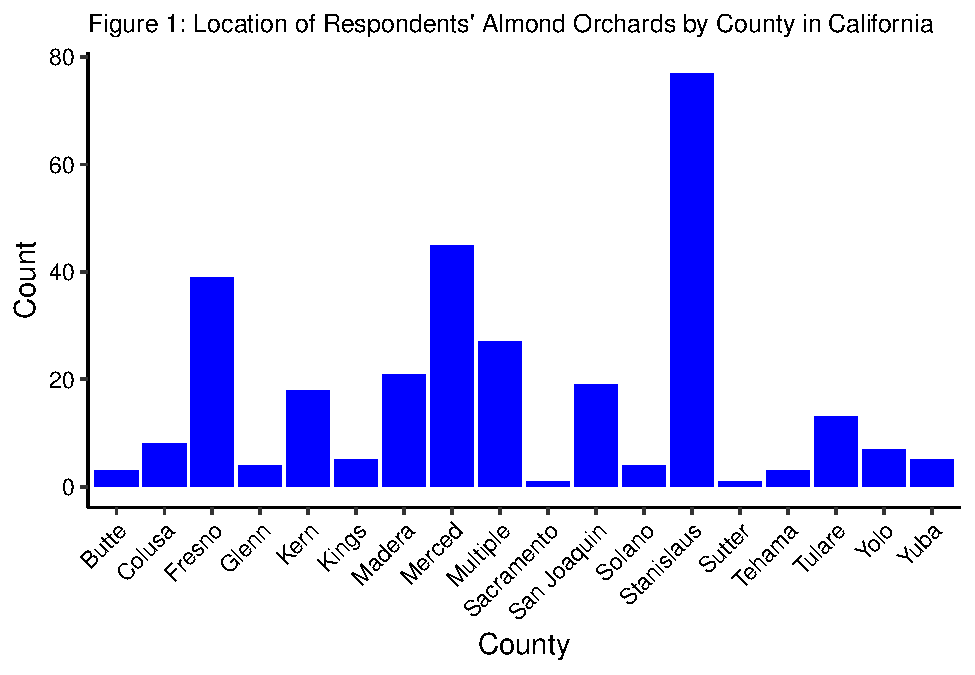
\includegraphics{Project_Template_files/figure-latex/location plots-1.pdf}
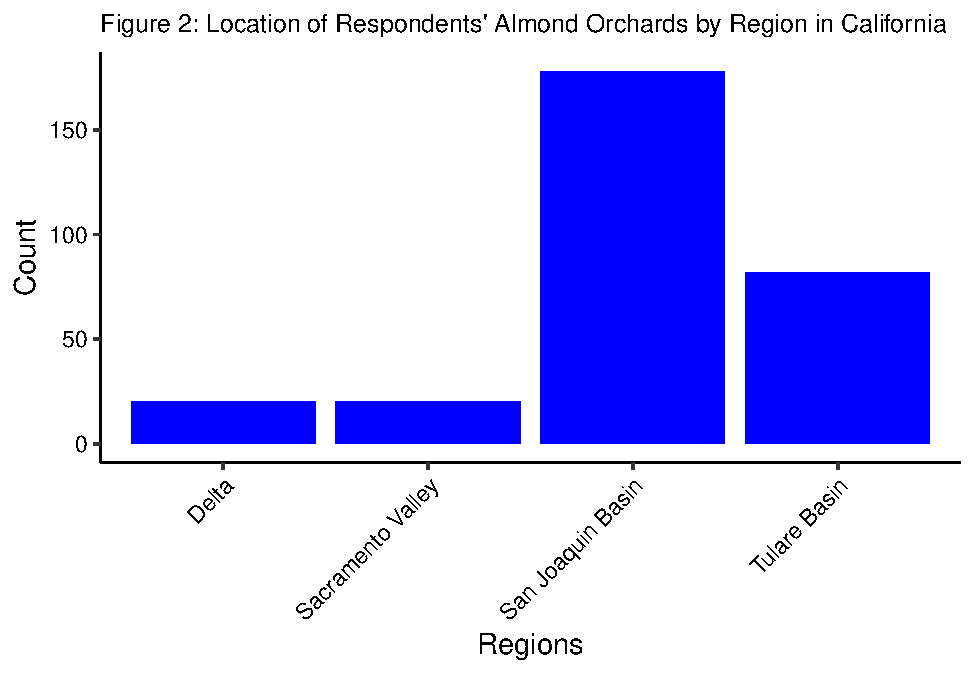
\includegraphics{Project_Template_files/figure-latex/location plots-2.pdf}

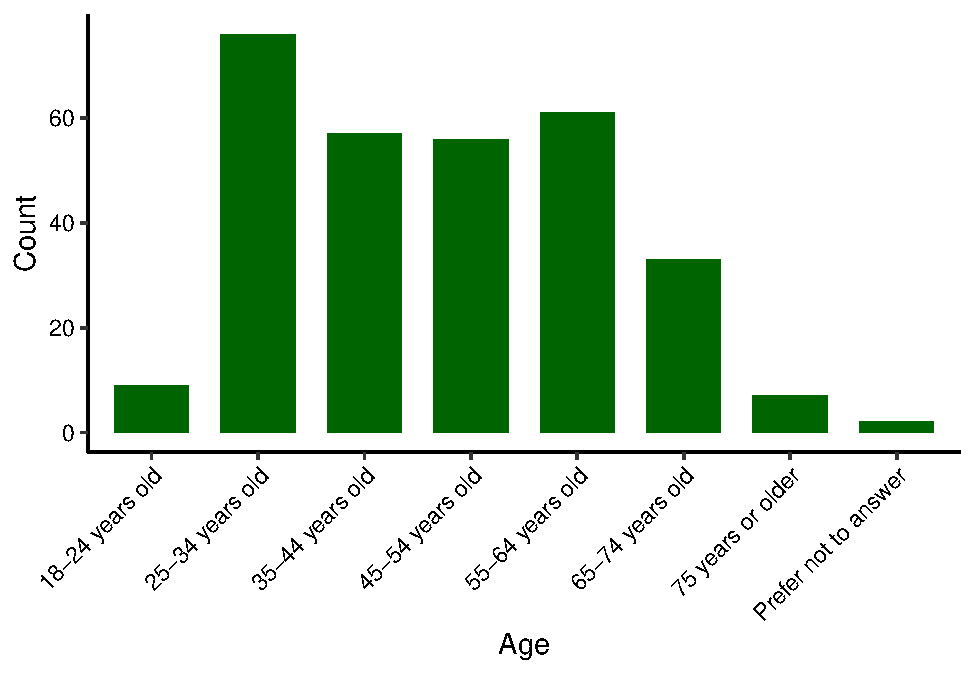
\includegraphics{Project_Template_files/figure-latex/respondent age-1.pdf}

\newpage

\section{Analysis}\label{analysis}

\subsection{\texorpdfstring{Question 1: THis part of analysis pertains
to question 1, etc. (helps organize relevant info for final
deliverable)}{Question 1:  THis part of analysis pertains to question 1, etc. (helps organize relevant info for final deliverable)}}\label{question-1-this-part-of-analysis-pertains-to-question-1-etc.-helps-organize-relevant-info-for-final-deliverable}

\subsection{Question 2:}\label{question-2}

\newpage

\section{Summary and Conclusions}\label{summary-and-conclusions}

\newpage

\section{References}\label{references}

\begin{itemize}
\tightlist
\item
  United States Department of Agriculture (USDA). (2019). 2018
  California Almond Acreage Report. California Department of Food and
  Agriculture. Retrieved from
  \url{https://www.nass.usda.gov/Statistics_by_State/California/Publications/Specialty_and_Other_Releases/Almond/Acreage/201904almac.pdf}
\end{itemize}

\end{document}
